\documentclass[12pt]{extarticle}
%Some packages I commonly use.
\usepackage[portuguese]{babel}
\usepackage{graphicx}
\usepackage{framed}
\usepackage[normalem]{ulem}
\usepackage{amsmath}
\usepackage{amsthm}
\usepackage{amssymb}
\usepackage{amsfonts}
\usepackage{enumerate}
\usepackage[utf8]{inputenc}
\usepackage{float}
\usepackage{gensymb}
\usepackage[top=1 in,bottom=1in, left=1 in, right=1 in]{geometry}
\usepackage{multirow}
\usepackage{caption}
\usepackage{subcaption}
\usepackage[utf8]{inputenc}

%A bunch of definitions that make my life easier
\newcommand{\matlab}{{\sc Matlab} }
\newcommand{\cvec}[1]{{\mathbf #1}}
\newcommand{\rvec}[1]{\vec{\mathbf #1}}
\newcommand{\ihat}{\hat{\textbf{\i}}}
\newcommand{\jhat}{\hat{\textbf{\j}}}
\newcommand{\khat}{\hat{\textbf{k}}}
\newcommand{\minor}{{\rm minor}}
\newcommand{\trace}{{\rm trace}}
\newcommand{\spn}{{\rm Span}}
\newcommand{\rem}{{\rm rem}}
\newcommand{\ran}{{\rm range}}
\newcommand{\range}{{\rm range}}
\newcommand{\mdiv}{{\rm div}}
\newcommand{\proj}{{\rm proj}}
\newcommand{\R}{\mathbb{R}}
\newcommand{\N}{\mathbb{N}}
\newcommand{\Q}{\mathbb{Q}}
\newcommand{\Z}{\mathbb{Z}}
\newcommand{\<}{\langle}
\renewcommand{\>}{\rangle}
\renewcommand{\emptyset}{\varnothing}
\newcommand{\grad}{$^\circ$}
\newcommand{\attn}[1]{\textbf{#1}}
\theoremstyle{definition}
\newtheorem{theorem}{Theorem}
\newtheorem{corollary}{Corollary}
\newtheorem*{definition}{Definition}
\newtheorem*{example}{Example}
\newtheorem*{note}{Note}
\newtheorem{exercise}{Exercise}
\newcommand{\bproof}{\bigskip {\bf Proof. }}
\newcommand{\eproof}{\hfill\qedsymbol}
\newcommand{\Disp}{\displaystyle}
\newcommand{\qe}{\hfill\(\bigtriangledown\)}
\setlength{\columnseprule}{1 pt}
\usepackage[utf8]{inputenc}

\title{Aula 1 - Termometria}
\author{Felipe Salvador}
\date{Atualizado em \today}

\begin{document}

\maketitle

Termometria é o estudo das propriedades (qualidades) térmicas (relacionadas a calor) das coisas, como temperatura, volume e pressão. Então, nessa primeira parte, veremos os conceitos mais básicos da termometria e como eles se relacionam.

\section{O que é Temperatura}
    Conceito: \textbf{Temperatura é o nível de agitação ou vibração média das moléculas que compõe um corpo, um líquido ou um gás.}
    
    Uma forma de entender a temperatura é pensando nos animais na natureza. Num inverno na Sibéria, os ursos e outros animais ficam recolhidos e em hibernação, não se movimentam muito e tendem a ficar juntos para aguentar o frio. Mas, já no verão, os animais ficam despertos e ativos, andam muito mais pelo ambiente que vivem, caçam, se reproduzem e assim por diante.
    
    A mesma coisa é com as moléculas. Temperaturas mais baixas, significa que as moléculas se movimentam, em média, muito pouco. Todavia, em temperaturas mais altas, as moléculas se movimentam bem mais, chegando a estarem bem agitadas, ao ponto de começarem a se distanciar bastante, como no caso da água que a 100\grad C ela se transforma em vapor.
    
    \section{Equilíbrio Térmico}
    Com isso, a temperatura se relaciona com a física a partir da chamado \textbf{Equilíbrio Térmico.} Ele nos diz que: \textbf{Se tivermos 2 corpos com temperaturas diferentes e eles entram em contato físico, a temperatura do 2 corpos será a mesma após um tempo.}
    
    Uma analogia que podemos fazer é quando temos uma aula com um professor muito empolgado. Depois de um tempo, vemos que estamos empolgados com a empolgação do professor.
    
    \section{Calor}
    Calor é dado como \textbf{O mecanismo de transferência de energia térmica de um corpo com mais energia térmica (maior temperatura) para um outro corpo que tem menos energia térmica (menor temperatura).}
    
    Aqui, calor é o processo de um corpo dar ou receber temperatura para um outro corpo. \textbf{Sempre quem dá temperatura é o corpo com maior temperatura e sempre quem recebe é o corpo com menor temperatura.}
    
    Portanto, \textbf{quem está dando calor para o outro é o corpo mais quente, enquanto quem recebe calor é o corpo mais frio.} Isso tudo acaba quando a temperatura dos dois corpos se iguala, pois ai não temos um corpo mais quente que o outro!
    
    \textbf{Quando o fluxo de calor de um corpo para outro para de acontecer, a gente diz que os dois corpos estão Equilíbrio Térmico, logo os 2 estão a uma mesma temperatura.}
    
    \begin{figure}[H]
        \centering
        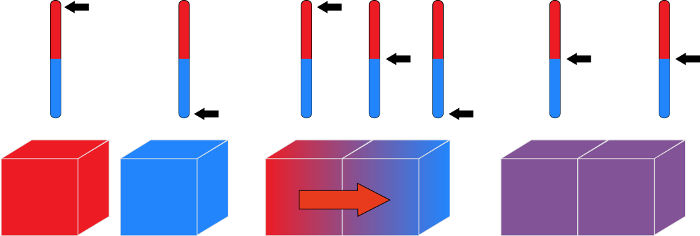
\includegraphics[width=0.7\textwidth]{equilibrio-termico.jpg}
        \caption{Esquema de como o Equilíbrio térmico ocorre. os 2 blocos com temperaturas diferente e quando entram em contato, acontece uma saída de calor do corpo mais quente em direção ao corpo mais frio, até que os 2 possuam a mesma temperatura.}
        \label{fig:exemplo_1}
    \end{figure}
    
    \section{Escalas de Temperatura}
    
    Em geral, trabalhamos com no máximo em 3 escalas.
    
    \begin{enumerate}
        \item \textbf{Escala Celsius} - é que usamos no nosso dia-a-dia e ela é bem intuitiva porque ela se baseia nas temperaturas que água se transforma em gelo e água se transforma em vapor:
        \begin{itemize}
            \item \textbf{Temperatura que a água se torna gelo:} 0\grad C;
            \item \textbf{Temperatura que a água se torna vapor d'água:} 100\grad C;
        \end{itemize}
        
        \item \textbf{Escala Fahrenheit} - é a escala mais usada nos EUA, atualmente, mas que era usada nos países que usavam o Sistema Imperial de Medidas. A escala foi construída de forma que o 0 fosse a temperatura de congelamento de uma solução de água, sal. Além disso, a 100 era a temperatura que uma pessoa estaria com febre. Em relação à temperatura em que a água se torna gelo ou vapor:
        \begin{itemize}
            \item \textbf{Temperatura que a água se torna gelo:} 32\grad F;
            \item \textbf{Temperatura que a água se torna vapor d'água:} 212\grad F;
        \end{itemize}
        
        \item \textbf{Escala Kelvin} - é a escala que a ciência usa, pois é uma escala somente positiva. Essa escala é construída de forma que a menor temperatura possível (o zero) é quando todas as moléculas estariam paradas, sem se movimentarem ou vibrarem. Pelos cálculos, descobriram que isso equivale à: $\mathbf{0K = -273,15\, ^\circ C}$, que no ensino médio, tomamos como: $\mathbf{0K = -273\,^\circ C}$. Em termos da água, a temperatura que a água vira gelo ou vapor é:
        \begin{itemize}
            \item \textbf{Temperatura que a água se torna gelo:} 273 K;
            \item \textbf{Temperatura que a água se torna vapor d'água:} 373 K;
        \end{itemize}
        
        Perceba que essa escala não tem \grad. Logo essa escala não é graduada, porque ela é uma escala absoluta, ou seja, não tem temperatura negativa!
    \end{enumerate}
    
    \section{Conversão entre escalas:}
    
    \begin{enumerate}
        \item \textbf{Celsius (\grad C) $\Longleftrightarrow$ Kelvin (K)}
        
        Existe uma fórmula que relaciona as 2:
        
        \begin{equation}
            T_{K} = T_{C} - 273
        \end{equation}
        \noindent em que $T_K$ é a temperatura em Kelvin, $T_{C}$ é a temperatura em Celsius.
        
        \item\textbf{Celsius (\grad C) $\Longleftrightarrow$ Fahrenheit (\grad F)}
        
        A fórmula que relaciona as duas escalas é dada por:
        
        \begin{equation}
            \frac{T_C}{5} = \frac{T_F - 32}{9} \iff T_F = 1,8*T_C + 32 
        \end{equation}
        \noindent em que $T_C$ é a temperatura em Celsius e $T_F$ é a temperatura em Fahrenheit.
        
        \item \textbf{Kelvin (K) $\Longleftrightarrow$ Fahrenheit (\grad F)}
        
        Basta usar a conversão de Kelvin para Celsius e depois usar a conversão de Celsius para Fahrenheit.
    \end{enumerate}
\end{document}
